\chapter{Vergleich der Varianten A und B}
Wir haben bereits einige Vor- und Nachteile der einzelnen Mikrogesten-Varianten diskutiert und möchten nun den tatsächlichen Unterschied praktisch testen. Für beide Varianten wird  ein Graph verwendet, um mit den Mikrogesten einen Buchstaben zu erkennen. Da der Graph sehr starr ist, muss die Mikrogesten-Erkennung bei jeder Eingabe eines Buchstaben das gleiche Resultat ergeben. Im Endeffekt besteht der Unterschied der beiden Varianten nur in der Mikrogesten-Erkennung.

\section{Vorgehensweise}
Die Varianten wurden folgendermassen verglichen:
\begin{itemize}
\item Wahl beliebiger Buchstaben.
\item Jeden Buchstaben theoretisch mit den beiden Varianten aufbauen.
\item Den Buchstaben 20x für jede Variante eingeben und die erkannten Mikrogesten loggen.
\item Die erkannten Mikrogesten mit den theoretischen vergleichen und die prozentuale Übereinstimmung errechnen
\item Den Mittelwert über alle Versuche berechnen. Dieser Wert kann dann zum Vergleich verwendet werden.
\end{itemize}

\section{Resultate}
Die kompletten in den Tests gewonnenen Daten sind im Anhang \ref{anhang_vergleich} zu finden. In den folgenden Abschnitten werden die Resultate jedoch noch untersucht und erläutert.

\subsection{Buchstabe 'm'}
Der Buchstabe 'm' lässt sich in beiden Varianten mit relativ wenigen Mikrogesten abbilden. In der Variante B kann dieser zum Beispiel aus nur drei Mikrogesten aufgebaut werden. Dies führt dazu, dass bei einer falsch erkannten Mikrogeste die Erkennungsrate schon drastisch sinkt. Im Gegenzug ist aber auch die Wahrscheinlichkeit höher, eine perfekte Erkennung zu erzielen.

In der Abbildung \ref{test_m} sind die Resultate der Testreihe abgebildet. Dort sieht man auch die starken Schwankungen der Erkennungsrate. In Tabelle \ref{test_avg} sind noch die Mittelwerte festgehalten: Es zeigt sich, dass Variante B trotz einiger schlechter Werte im Schnitt eine bessere Erkennung bietet.

\begin{figure}[h!]
  \centering
    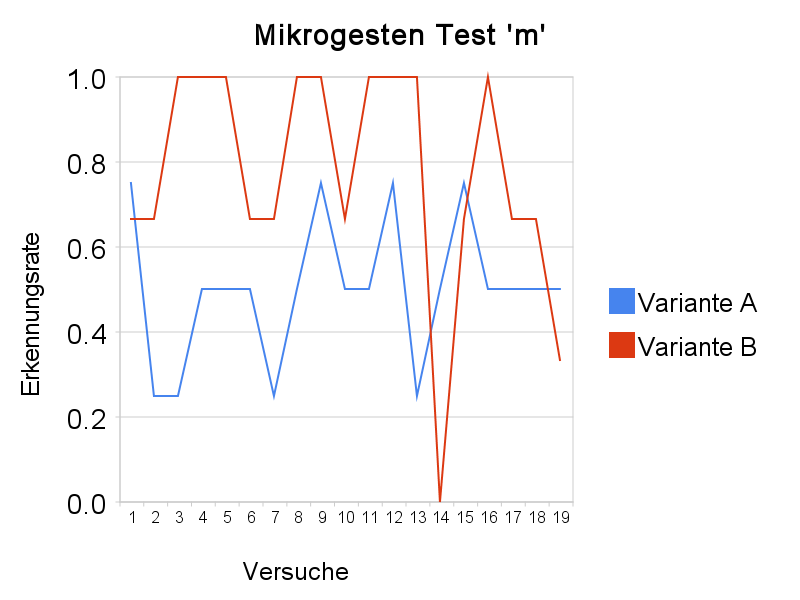
\includegraphics[scale=0.4]{./img/mikrogesten_test_m.png}
  \caption{Resultat der Versuchsreihe mit dem Buchstaben 'm'.  }
  \label{test_m}
\end{figure}

\begin{table}[h!]
  \begin{center}
    \begin{tabular}{l | c |  c }
    \emph{Buchstabe} &  \emph{Variante A} &  \emph{Variante B} \\ \hline
    m & 51\% & 78\% \\ \hline
    k & 45\% &  88\% \\
    \end{tabular}
  \end{center}
  \caption{Durchschnittliche Erkennungsrate der beiden Versuche}
  \label{test_avg}
\end{table}

\subsection{Buchstabe 'k'}
In diesem Test wurde die Erkennungsrate des Buchstaben 'k' in kursivschreibweise getestet. Dies ist der Buchstaben, der aus den meisten Mikrogesten aufgebaut wird und deshalb auch der komplexeste ist. 

Die mittlere Erkennungsrate ist in Tabelle \ref{test_avg} festgehalten und die einzelnen Werte in Abbildung \ref{test_k}. Interessanterweise schneidet der komplexe Buchstabe 'k' besser ab als der einfache Buchstabe 'm'. Dies kann wie folgt erklärt werden: Es gibt eine Reihe von einfachen Buchstaben, die alle aus zwei bis vier Mikrogesten bestehen. Man kann also im Graph nicht viele Varianten eines einzelnen Buchstabens zulassen, da ansonsten schnell Überschneidungen mit anderen Buchstaben entstehen. Wenn nun schon nur eine einzige Mikrogeste falsch erkannt wurde, kann dies bereits zu einem falschen Resultat führen.

Komplexe Buchstaben hingegen unterscheiden sich im Mikrogesten-Aufbau stark von den anderen Buchstaben. Dadurch kann man selbst dann noch den korrekten Buchstaben finden, wenn einige der Mikrogesten nicht übereinstimmen.

Bei Variante A schnitt 'k' schlechter ab als 'm', was daran liegt, dass die kursive Version von 'k' sehr viele mögliche Schreibweisen besitzt. Da Variante A zwischen starken und schwachen Krümmungen unterscheidet, ist es bei diesem Buchstaben relativ  zufällig, ob jetzt eine starke oder eine schwache Krümmung erkannt wird. Durch den oben genannten Effekt der komplexen Buchstaben ist eine Erkennung aber trotzdem noch möglich.

\begin{figure}[h!]
  \centering
    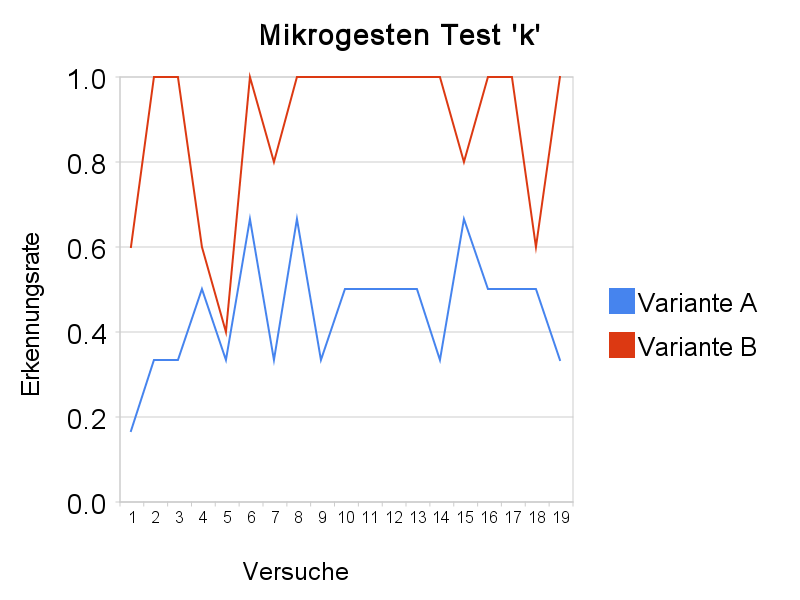
\includegraphics[scale=0.4]{./img/mikrogesten_test_k.png}
  \caption{Resultat der Versuchsreihe mit dem Buchstaben 'k'.  }
  \label{test_k}
\end{figure}

\section{Die perfekte Mikrogesten-Variante}
Aus den bisherigen Erkenntnissen und Tests können folgende Schlüsse gezogen werden:

\begin{itemize}
 \item Die Mikrogesten müssen so definiert sein, dass sie mit einem möglichst einfachen Algorithmus erkannt werden können.
 \item Die Mikrogesten müssen sich so stark wie möglich voneinander Unterscheiden. Eine starke Unterscheidung sollte automatisch auch zu einer einfachen Erkennung führen.
 \item Es ist nicht von Vorteil, die Buchstaben mit möglichst wenigen Mikrogesten aufzubauen. Paradoxerweise kann dies die Erkennungsrate verschlechtern.
\item Nach Erfahrungswerten ist eine Mikrogestenzahl von vier bis sechs am besten geeignet. Die Erkennungsrate der Mikrogesten ist jedoch viel wichtiger als die durchschnittlich benötigte Mikrogestenzahl pro Buchstaben!
\end{itemize}

\section{Fazit}
Variante B schneidet bei der Erkennung besser ab, ist jedoch auch nicht perfekt. Vor allem bei den Kleinbuchstaben hat man immer noch das Problem, dass ähnliche Buchstaben schwer zu unterscheiden sind. Die Ähnlichkeit ist allerdings von der Schrift gegeben und lässt sich nicht ändern. Deshalb ist die sinnvollste Optimierung die Überarbeitung der Mikrogesten-Erkennungsalgorithmen. Dort besteht immer noch sehr viel Verbesserungsbedarf: Wie beim Test gesehen, werden selbst einfache Buchstaben nur in 78\% der Fälle erkannt.